\chapter{Численное решение задачи с учётом роста трещин автоГРП в длину} \label{ch3}


С помощью метода Ньютона проведено решение поставленной в первом разделе задачи.
Рассматривались 3 одинаковые трещины гидроразрыва.
Результаты представлены на рис. \ref{fig:results1}.

\begin{figure}[H]
	\adjustbox{minipage=1.3em,valign=t}{\subcaption{}\label{fig:p_0(q_0)}}%
	\begin{subfigure}[t]{\dimexpr.5\linewidth-1.3em\relax}
		\centering
		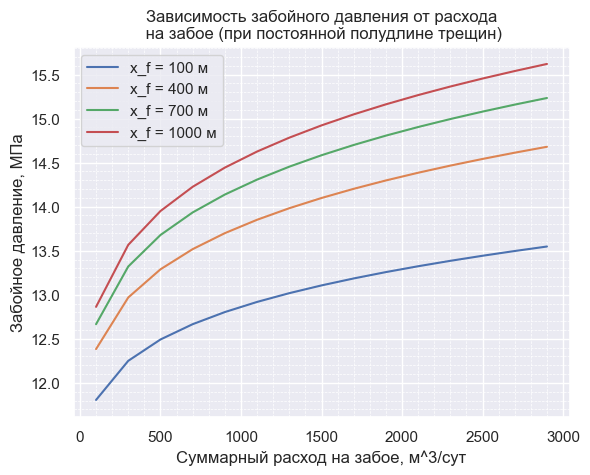
\includegraphics[width=.95\linewidth,valign=t]{images/p_0(q_0).png}
	\end{subfigure}
\hfill %выровнять по ширине
	\adjustbox{minipage=1.3em,valign=t}{\subcaption{}\label{fig:p_0(x_f)}}%
	\begin{subfigure}[t]{\dimexpr.5\linewidth-1.3em\relax}
		\centering
		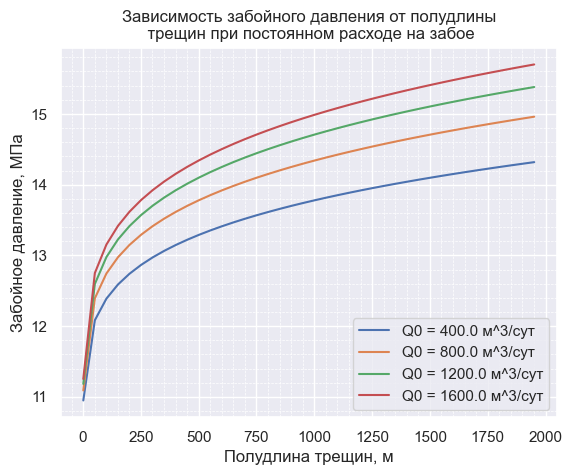
\includegraphics[width=.95\linewidth,valign=t]{images/p_0(x_f).png}
	\end{subfigure}
\captionsetup{justification=centering} %центрировать
\caption{Зависимости забойного давления от основных параметров задачи: {\itshape a} --- от суммарного расхода на забое; {\itshape b} --- от полудлины трещин} 
\label{fig:results1}
\end{figure}

Далее для учёта роста трещин автоГРП в длину было проведено совмещение уравнений законов Кирхгофа \eqref{1_1} и \eqref{1_2} с формулой Кёнинга \cite{koning}:
\beq
x_f=\frac{q\mu\sqrt{\pi\kappa t}}{2\pi kh\Delta p},
\eeq
где $x_f$ -- полудлина трещины автоГРП;\newline
$q$ -- расход закачиваемой жидкости на трещине;\newline
$\mu$ -- вязкость закачиваемой жидкости;\newline
$\kappa$ -- пьезопроводность пласта;\newline
$k$ -- проницаемость пласта;\newline
$h$ -- эффективная проницаемая толщина (мощность) пласта;\newline
$\Delta p$ -- средняя по времени разница между пластовым и забойным давлениями;\newline
$t$ -- время закачки.

Результаты моделирования представлены на рис. \ref{fig:results2}.
 
\begin{figure}[H] 
\center
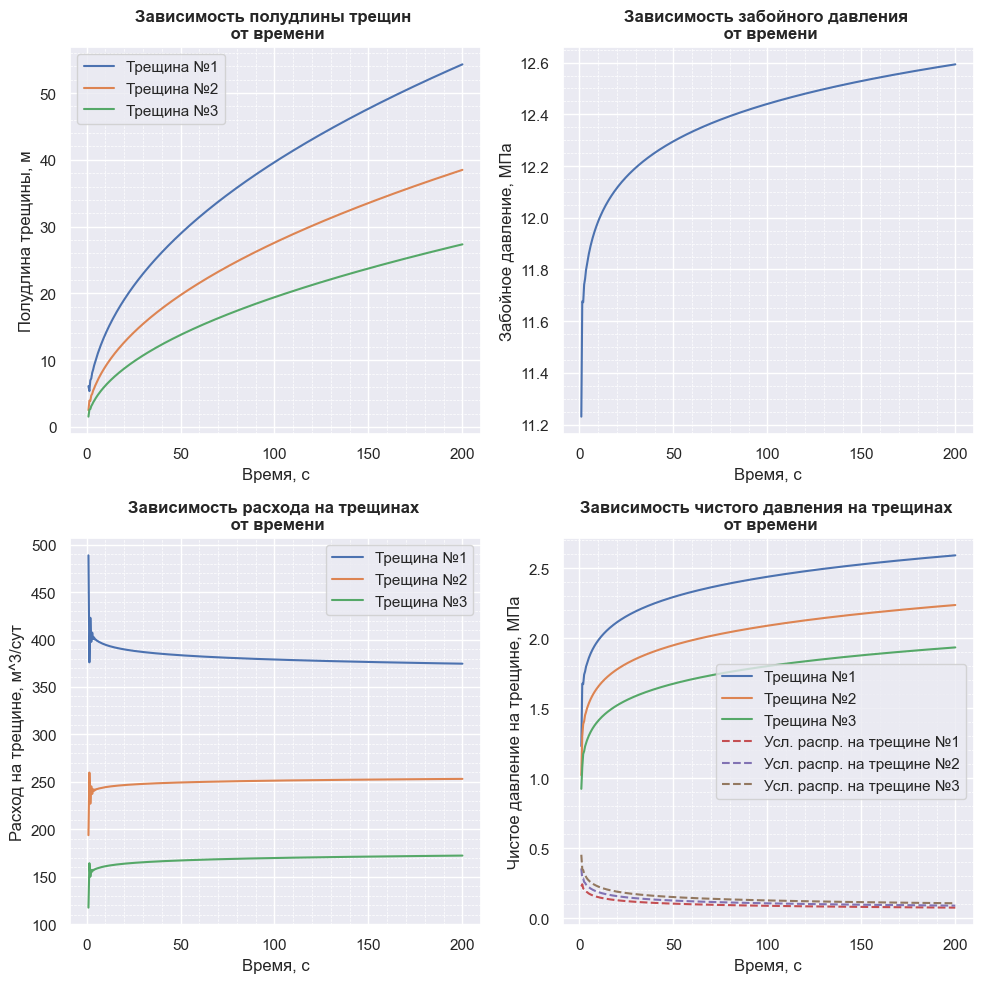
\includegraphics[width=\linewidth]{images/Kirchhoff+Koning.png}
\caption{Результаты решения поставленной задачи} 
\label{fig:results2}  
\end{figure}

В проведённом численном эксперименте трещины отличаются друг от друга количеством и диаметром перфораций.\newline
У трещины 1: количество перфораций 32, диаметр перфораций 0.02 м.\newline
У трещины 2: количество перфораций 2, диаметр перфораций 0.01 м.\newline
У трещины 3: количество перфораций 1, диаметр перфораций 0.01 м.
\\

Код решения представлен по ссылке: \url{https://github.com/mualal/hydrofracturing/blob/master/notebooks/02_fractures_growth_with_Koning.ipynb}

Из графиков на рис. \ref{fig:results2} видим, что большую часть потока забирает на себя трещина с лучшими перфорациями.
Эта же трещина лидирует по скорости роста.

Также видим, что при росте трещин требуется всё большее забойное давление для того, чтобы поддерживать этот рост.

При выбранных входных параметрах построенной модели чистое давление в каждой из трещин существенно превышает давления критерия распространения, следовательно, при достаточно высоком забойном давлении все трещины будут расти одновременно.
